\chapter{Introduction}
\lecture{1}{13/1}

\begin{definition}[Machine learning]
    \textbf{Machine learning} is a study of algorithms and models
    that computers use to perform specific tasks without being explicitly programmed.
\end{definition}
It allows us to
\begin{enumerate}
    \item reduce time spent programming;
    \item customise products for users; and
    \item to solve problems that you have no idea how to do by hand.
\end{enumerate}

\begin{example}
    Machine learning is used to generate things like:
    \begin{enumerate}
        \item netflix recommendations; and
        \item twitter personalised timelines
    \end{enumerate}
    and has also been applied to
    \begin{enumerate}
        \item logistics; and
        \item self-driving cars.
    \end{enumerate}
\end{example}

We can redefine machine learning with a more mathematical approach.

\begin{definition}[Machine learning]
    \textbf{Machine learning} is the study of algorithms
    that improve their performance $P$ at some task $T$ with experience $E$.
\end{definition}

\begin{definition}[Supervised learning]
    \textbf{Supervised learning} is the task of learning a function
    that maps an input to an output based on example input-output pairs.
\end{definition}

\begin{example}
    Consider an algorithm that will learn to recognise pictures of bees
    which is \emph{trained} on pictures of bees each with a label
    saying whether or not the picture is a bee.
    This is a supervised learning algorithm.
\end{example}

\begin{definition}[Unsupervised learning]
    \textbf{Unsupervised learning} is the task of learning patterns in data
    with no pre-existing labels (and with minimum human supervision).
\end{definition}

\begin{figure}
    \centering
    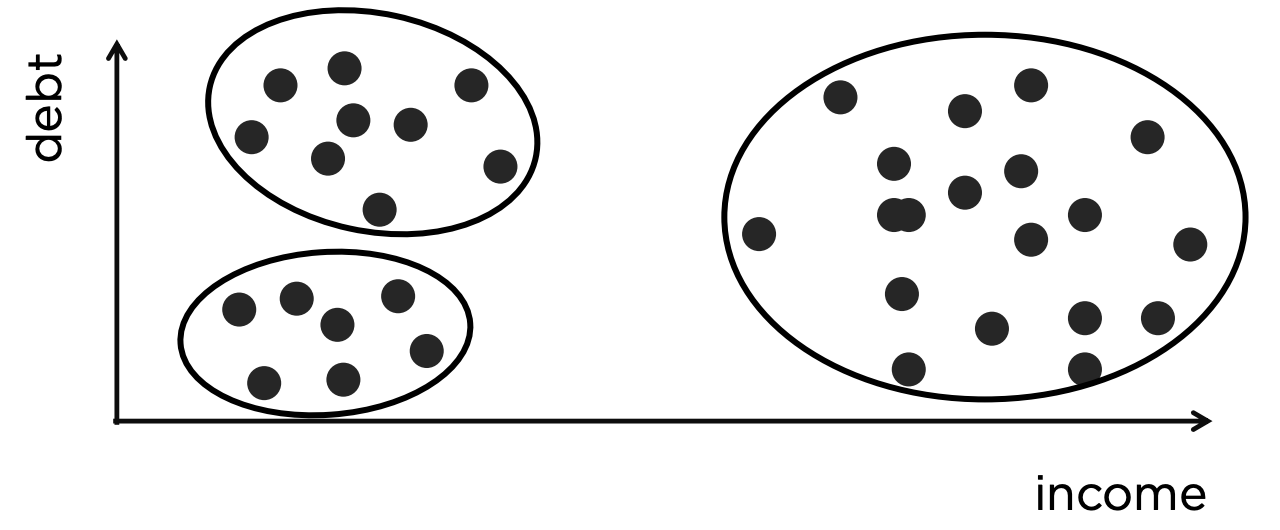
\includegraphics[width=0.8\linewidth]{images/unsupervised-learning.png}
    \caption{An example of a unsupervised learning model clustering data points together.}
    \label{fig:unsupervised-learning}
\end{figure}

\begin{remark}
    Unsupervised learning models will cluster the data 
    into groups where it thinks that all the data in a group
    are more similar to the other data in its group than to 
    the rest of the dataset, as shown in 
    Figure \ref{fig:unsupervised-learning}.
\end{remark}

\begin{definition}[Reinfornced learning]
    \textbf{Reinfornced learning} (RL) is a category of machine learning where
    \emph{software agent} take \emph{actions} in an environment
    based on some notion of cumulative reward.
\end{definition}

A \textbf{label} is the variable we are predicting.
\textbf{Features} are input variables that describe our data.
An \textbf{example} is an instance of data, which can be labelled or unlabelled.
A \textbf{model} is a software agent that maps examples to labels.

\begin{example}
    Suppose we have a data set with $n$ features in $\R^n$.
    Let $S$ be a set of labels.
    Then $\bm x = (x_1, x_2, \ldots, x_n) \in \R^n$ denotes a specific
    unlabelled example where $x_i$ is the $i$th feature of the example.
    $(\bm x, s) \subset \R^n \times S$ denotes a labelled example.
    Then a function $f: \R^n \to S$ denotes a model which takes an
    unlabelled example and produces a label.
    Now consider $S = \R$.
    We can denote a $D$ dataset of $k$ units (examples) as
    \[
        D = \{y_i, x_{i1}, x_{i2}, \ldots, x_{in}\}_{i=1}^k
    \]
    where $y_i$ is a label and $x_ij$ is the $j$th feature in the $i$th unit.
\end{example}
